\subsection{Cluster Analysis Results Visualization}
\label{sec:cluster}

Figure~\ref{fig:Cytoscape_Cluster_2} from Section~\ref{sec:dataset_description} shows cluster graph specific structure: it is very high, unbalanced and has not so deep sub-parts.
It is possible to use this disadvantage as advantage and abstract sub-parts to reduce drawing area.
For this we need to extract those nodes and edges that form the longest path of the cluster graph - ,,backbone''. Figure~\ref{fig:cluster_visualisation} shows the algorithm step by step.
Backbone vertices are filled with yellow and are shown in Figure~\ref{fig:cluster_visualisation_algorithm_1}.
Next step is to abstract branches into groups. Group size is scaled according to amount of elements inside.

\begin{figure}[h!]
\centering
\subfloat[Backbone and branches]{
    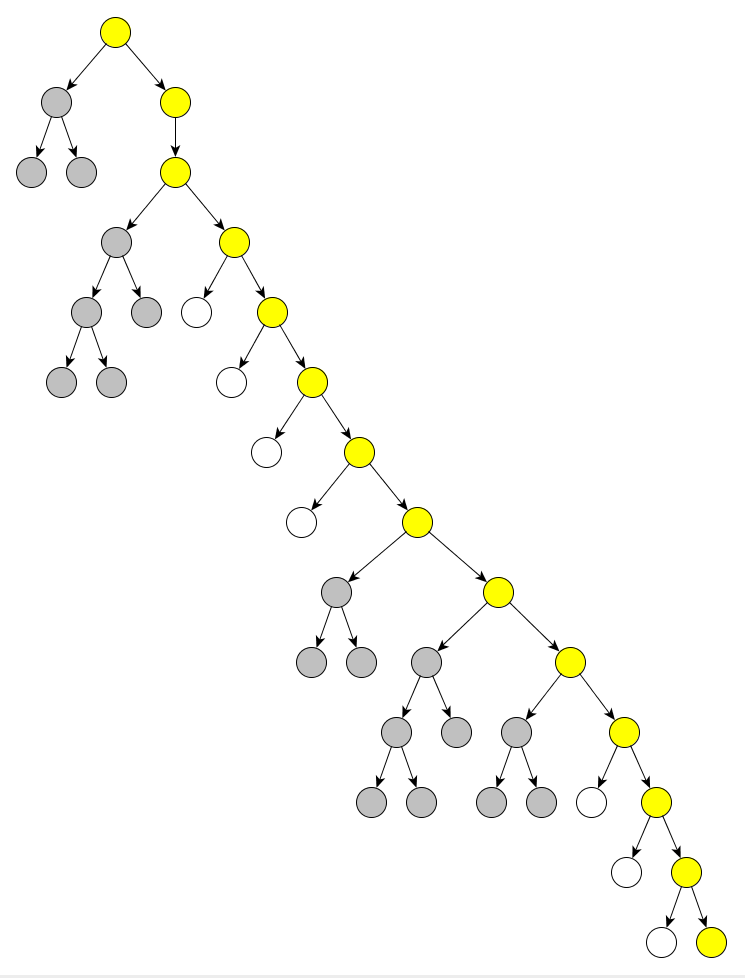
\includegraphics[scale=0.15]{pictures/cluster_visualisation_algorithm_1.png}
    \label{fig:cluster_visualisation_algorithm_1}
}
\subfloat[Abstract branches into groups]{
    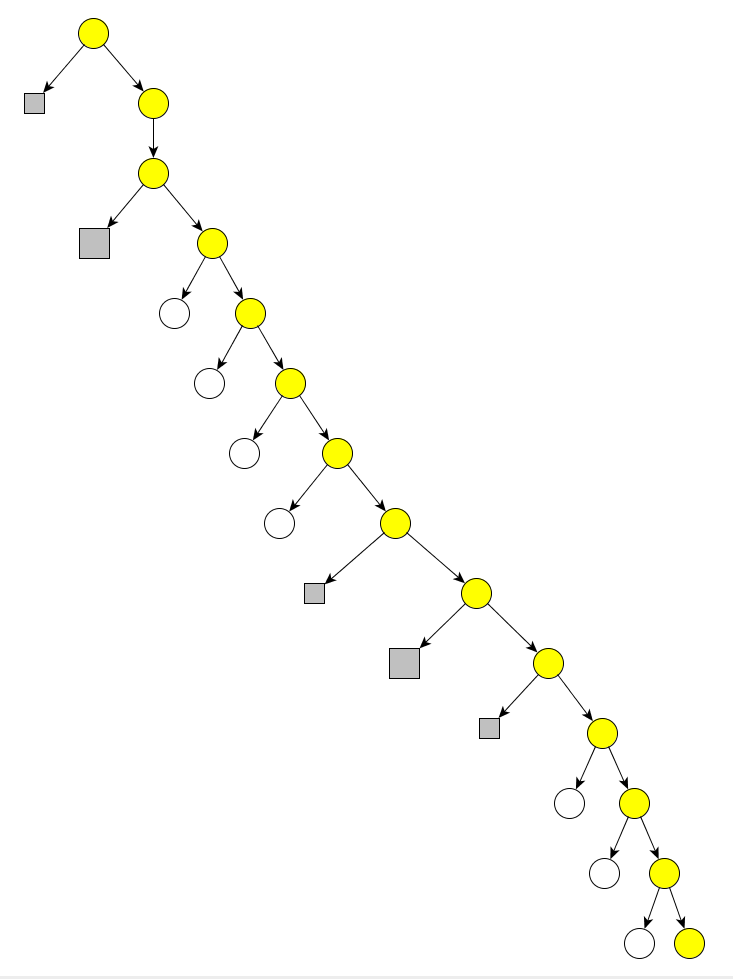
\includegraphics[scale=0.15]{pictures/cluster_visualisation_algorithm_2.png}
    \label{fig:cluster_visualisation_algorithm_2}
}
\subfloat[Scale group size]{
    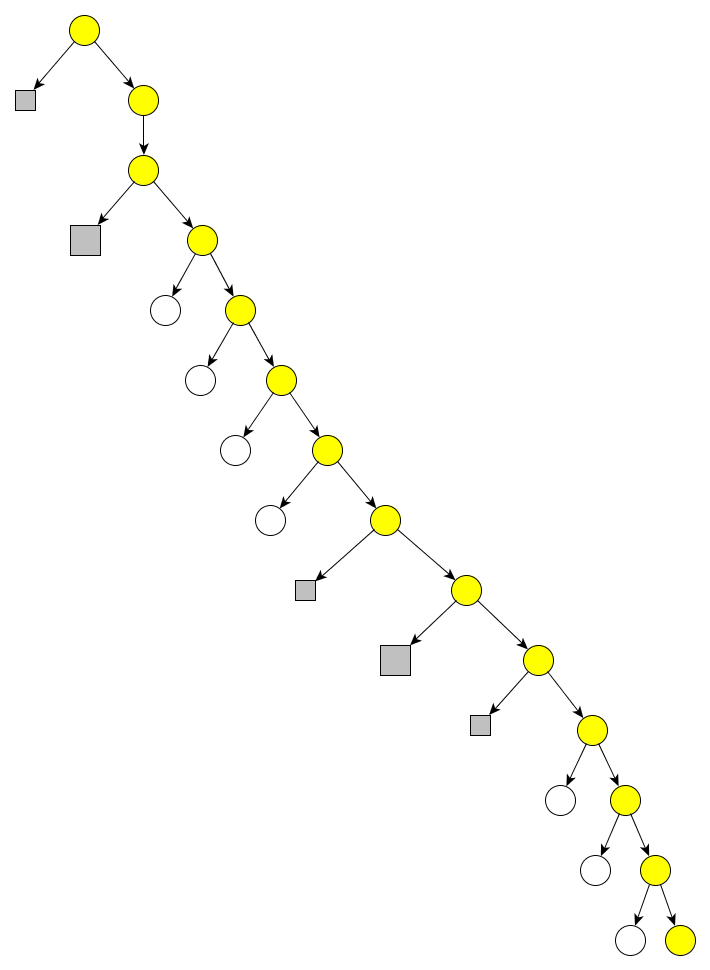
\includegraphics[scale=0.15]{pictures/cluster_visualisation_algorithm_3.png}
    \label{fig:cluster_visualisation_algorithm_3}
}
\caption{Cluster Visualization algorithm}
\label{fig:cluster_visualisation_algorithm}
\end{figure}

The last step is to represent backbone as a spiral, thus preserving space and giving a possibility to show the complete tree in one view.
Figure~\ref{fig:cluster_visualisation_algorithm_4} shows how it works.

\begin{figure}[h!]
\centering
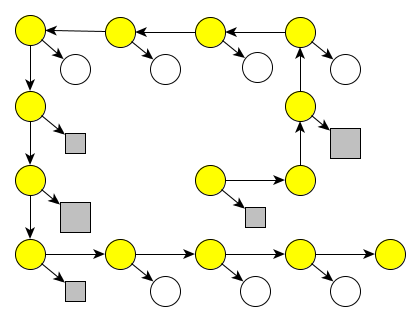
\includegraphics[scale=0.5]{pictures/cluster_visualisation_algorithm_4.png}
\caption{,,Rectangular Spiral Layout''}
\label{fig:cluster_visualisation_algorithm_4}
\end{figure}

Then backbone formed as rectangular spiral with a root in the center and moving in clockwise direction.
Figure~\ref{fig:cluster_visualisation} shows complete visualization result for the real cluster tree.
This approach reuses space as much as possible and still gives overview of location of the highlighted vertices in cluster hierarchy -- how far it is from the root.

\begin{figure}[h!]
\centering
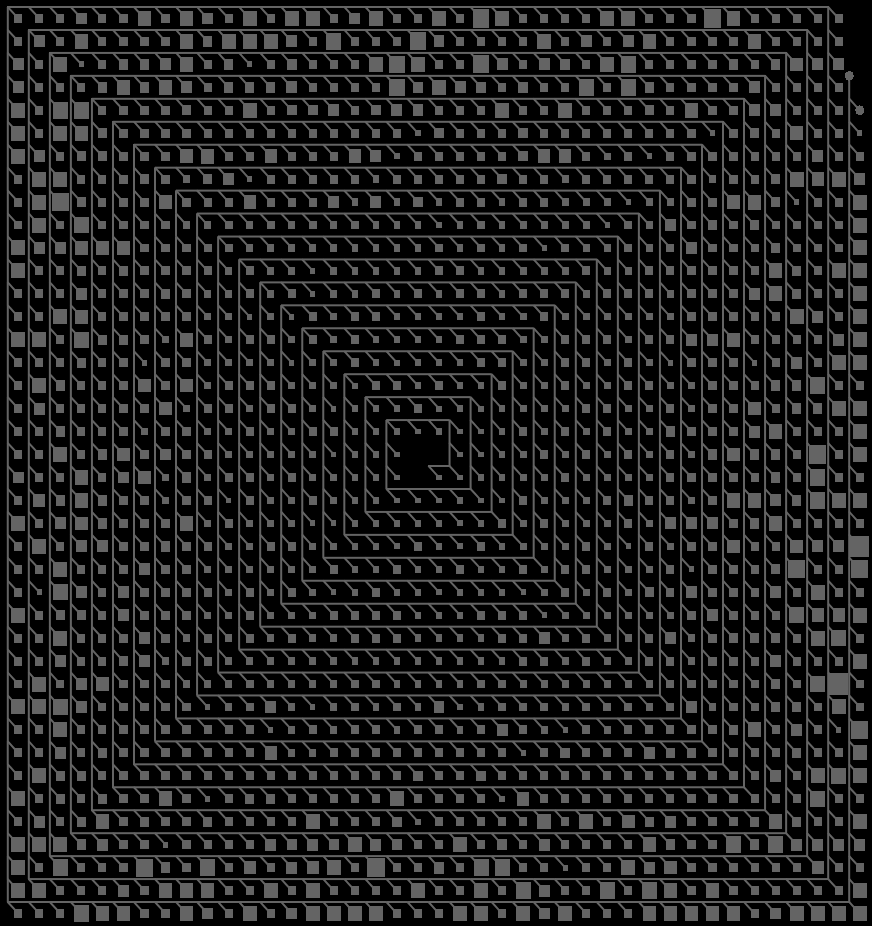
\includegraphics[scale=0.4]{pictures/cluster_spiral_visualisation.png}
\caption{Rectangular spiral Cluster graph visualization}
\label{fig:cluster_visualisation}
\end{figure}

It is possible to explore sub-parts (rectangles) of the Cluster graph using ,,lens''. User can interactively choose any sub-part and the lens with inner content will appear.
There are two different lens layouts: polar (Figure~\ref{fig:lens_polar}) and HV-tree (Figure~\ref{fig:lens_tree}).
Polar lens layout is based on the algorithm used for initial visualization of the Cluster graph, the algorithm was explained earlier in Section~\ref{sec:probe}.
Both implementations are made by our own and are not based on any third party source code.

\begin{figure}[h!]
\centering
\subfloat[Polar lens layout]{
    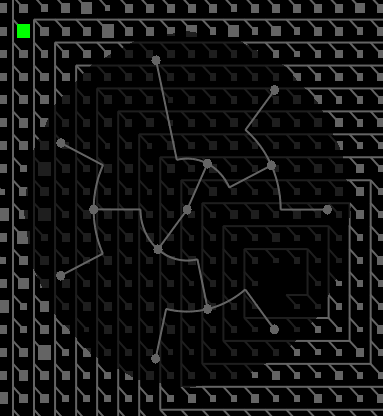
\includegraphics[scale=0.5]{pictures/lens_polar.png}
    \label{fig:lens_polar}
}
\\
\subfloat[HV-tree lens layout]{
    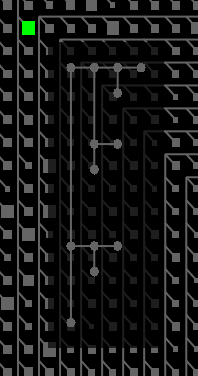
\includegraphics[scale=0.5]{pictures/lens_tree.png}
    \label{fig:lens_tree}
}
\caption{Different lens layouts}
\end{figure}

